\documentclass{beamer} 
\usepackage{amsmath} 
\usepackage{xcolor} 
\usepackage{xpatch} 
\usepackage{cancel} 
\usepackage{enumitem} 
\usepackage{pgfplots}
\usepackage{framed}
\title{Positive and Negative Intervals of Polynomials} 
\pgfplotsset{width = 10cm, compat = 1.9}
\usepgfplotslibrary{external, groupplots}
\tikzexternalize


\begin{document}
	\frame{
	\titlepage
}
	\frame{
		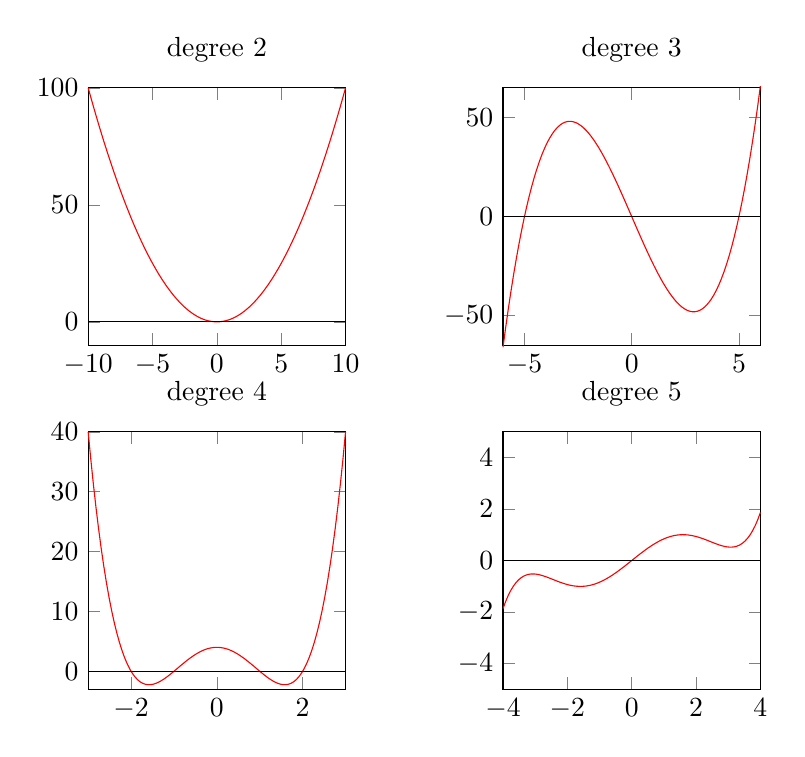
\begin{tikzpicture}
   \begin{groupplot}[
        group style = {group size = 2 by 2, vertical sep = 1.1cm, horizontal sep = 2cm},
        width=0.4\linewidth,
        height=0.4\linewidth,
        ]

        \nextgroupplot[
                title = degree 2,
                xmin = -10,
                xmax = 10,
                ymin = -10,
                ymax = 100,
                ymode = linear,
                clip = false,
        ]
        \addplot [
		domain = -10:10,
		samples = 100,
		color = red,
		]
	   {x^2};
	\addplot [
		domain = -10:10,
		samples = 100,
		color = black,
		 ]
		{0};
        
	   \nextgroupplot[
                title = degree 3,
                xmin = -6,
                xmax = 6,
                ymin = -65,
                ymax = 65,
                ymode = linear,
                clip = false,
        ]
        \addplot [
		domain = -6:6,
		samples = 100,
		color = red,
		]
	   {x*(x - 5)*(x + 5)};

	\addplot [
		domain = -6:6,
		samples = 100,
		color = black,
		 ]
		{0};
        
	   \nextgroupplot[
                title = degree 4,
                xmin = -3,
                xmax = 3,
                ymin = -3,
                ymax = 40,
                ymode = linear,
                clip = false,
        ]
        \addplot [
		domain = -3:3,
		samples = 100,
		color = red,
		]
	   {(x - 2)*(x - 1)*(x + 1)*(x + 2)};

	\addplot [
		domain = -3:3,
		samples = 100,
		color = black,
		 ]
		{0};

        \nextgroupplot[
                title = degree 5,
                xmin = -4,
                xmax = 4,
                ymin = -5,
                ymax = 5,
                ymode = linear,
                clip = false,
        ]
        \addplot [
		domain = -4:4,
		samples = 100,
		color = red,
		]
	   {x-(x^3/6) + x^5 / 120};

	\addplot [
		domain = -4:4,
		samples = 100,
		color = black,
		 ]
		{0};

   \end{groupplot}
\end{tikzpicture}


}
	\frame{
		\begin{tikzpicture}
\begin{axis}[
    axis lines = left,
    xlabel = $x$,
    ylabel = {$f(x)$},
]

%Single point
\addplot[domain = -10:10, mark = *, color = green] coordinates {(0,0)};
\addplot[domain = -10:10, mark = *, color = green] coordinates {(1,1)};
\addplot[domain = -10:10, mark = *, color = green] coordinates {(2,4)};
\addplot[domain = -10:10, mark = *, color = green] coordinates {(3,9)};
\addplot[domain = -10:10, mark = *, color = green] coordinates {(4,16)};
\addplot[domain = -10:10, mark = *, color = green] coordinates {(5,25)};
\addplot[domain = -10:10, mark = *, color = green] coordinates {(6,36)};
%red parabola
\addplot [
    domain=-10:10,
    samples=100,
    color=red,
]
{x^2};
\addlegendentry{$x^2$}
\end{axis}
\end{tikzpicture}


		}
	\frame{
		$x^3 - 25x$
		}
	\frame{
		$f(x) = x^3 - 25x = 0$\pause\\
		$x(x^2 - 25) = 0$\pause\\
		$x \hspace{1cm} 5$\pause\\
		$x \hspace{1cm} -5$\pause\\
		$-5x\pause + 5x = 0$\pause\\
		$x(x + 5)(x - 5) = 0$\pause\\
		$f(0) = (0)(5)(-5) = 0$\pause\\
		$f(-5) = (-5)(0)(-10) = 0$\pause\\
		$f(5) = (5)(10)(0) = 0$\pause\\
		}
	\frame{
		\begin{tikzpicture}
\begin{axis}[
    axis lines = left,
    xlabel = $x$,
    ylabel = {$f(x)$},
]
%red parabola
\addplot [
    domain=-6:6,
    samples=100,
    color=red,
]
{x*(x - 5)*(x + 5)};
\addlegendentry{$x^3 - 25x$}
\end{axis}
\end{tikzpicture} 

		}
	\frame{
		\begin{tikzpicture}
\begin{axis}[
    axis lines = left,
    xlabel = $x$,
    ylabel = {$f(x)$},
]

%Single point
\addplot[domain = -6:6, mark = *, color = green] coordinates {(0,0)};
\addplot[domain = -10:10, mark = *, color = green] coordinates {(-5,0)};
\addplot[domain = -10:10, mark = *, color = green] coordinates {(5,0)};
\addplot[domain = -10:10, mark = *, color = green] coordinates {(-2,42)};
 \addplot [
                domain = -6:6,
                samples = 100,
                color = black,
                 ]
                {0};%\addplot[domain = -10:10, mark = *, color = green] coordinates {(2,-42)};
%red parabola
%\addplot [
%    domain=-10:10,
%    samples=100,
%    color=red,
%]
%{x^2};
%\addlegendentry{$x^2$}
\end{axis}
\end{tikzpicture}


		}
	\frame{
		\begin{tikzpicture}
\begin{axis}[
    axis lines = left,
    xlabel = $x$,
    ylabel = {$f(x)$},
]

%Single point
\addplot[domain = -6:6, mark = *, color = green] coordinates {(0,0)};
\addplot[domain = -10:10, mark = *, color = green] coordinates {(-5,0)};
\addplot[domain = -10:10, mark = *, color = green] coordinates {(5,0)};
\addplot[domain = -10:10, mark = *, color = green] coordinates {(-2,42)};
\addplot[domain = -10:10, mark = *, color = green] coordinates {(2,-42)};
 \addplot [
                domain = -6:6,
                samples = 100,
                color = black,
                 ]
                {0};%red parabola
%\addplot [
%    domain=-10:10,
%    samples=100,
%    color=red,
%]
%{x^2};
%\addlegendentry{$x^2$}
\end{axis}
\end{tikzpicture}


		}
	\frame{
		\begin{tikzpicture}
\begin{axis}[
    axis lines = left,
    xlabel = $x$,
    ylabel = {$f(x)$},
]

%Single point
\addplot[domain = -6:6, mark = *, color = green] coordinates {(0,0)};
\addplot[domain = -6:6, mark = *, color = green] coordinates {(-5,0)};
\addplot[domain = -6:6, mark = *, color = green] coordinates {(5,0)};
\addplot[domain = -6:6, mark = *, color = green] coordinates {(-2,42)};
\addplot[domain = -6:6, mark = *, color = green] coordinates {(2,-42)};
\addplot[domain = -6:6, mark = *, color = green] coordinates {(6,66)};
\addplot[domain = -6:6, mark = *, color = green] coordinates {(-6,-66)};

\addplot [
    domain=-6:6,
    samples=100,
    color=red,
]
{x^3 - 25 * x};
\addlegendentry{$x^3 - 25x$}
 \addplot [
                domain = -6:6,
                samples = 100,
                color = black,
                 ]
                {0};
\end{axis}
\end{tikzpicture}


		}
\end{document}
